\documentclass{article}

\usepackage[dvips]{graphicx}
\usepackage{wrapfig}
\usepackage{color}
\usepackage{ascmac}
% \usepackage{makeidx}

\setlength{\oddsidemargin}{0.5cm}
\setlength{\evensidemargin}{0.5cm}
\setlength{\textwidth}{423pt}
\setlength{\topmargin}{0pt}

\title{Curriculum Vitae}
\author{Rintaro Saito\\ \\

\includegraphics[scale=0.5]{logo_ucsd1}\\
University of California, San Diego\\
Departments of Medicine and Bioengineering
}

\begin{document}

\maketitle

\section{Profile}

\begin{minipage}{0.6\hsize}
\begin{tabular}{ll}
Family Name   & Saito \\
Given Name    & Rintaro \\
Gender        & Male \\
Date of Birth & November 5, 1972 \\
Nationality   & Japanese \\
Address       & San Diego, California, U.S.A.\\
Marital Status & Married\\
Degree        & Ph.D. (Keio University, 2000)\\
Affiliation   & {\small University of California, San Diego}\\
              & {\small Departments of Medicine and Bioengineering}\\
              & {\small (Postal address: 9500 Gilman Drive}\\
              & {\small La Jolla, CA 92093-0688)}\\
Title         & Visiting Faculty \\
Research Field & Bioinformatics\\
Research Interests & Computational genomic analyses (especially on non-coding regions)\\
                   & Interactome analyses\\
Tel           & +1-858-822-4667\\
Fax           & +1-858-822-4246\\
E-Mail        & risaito@ucsd.edu\\
Web Page      & http://www.bioinfo.sfc.keio.ac.jp/class/bioinfo-a/WEB\verb+_+RS\\
Skype ID      & golgo8028\\
Hobby         & Skiing, Driving, GO (Traditional Asian board game)
\end{tabular}
\end{minipage} % No open line below!
\begin{minipage}{0.4\hsize}
\begin{center}
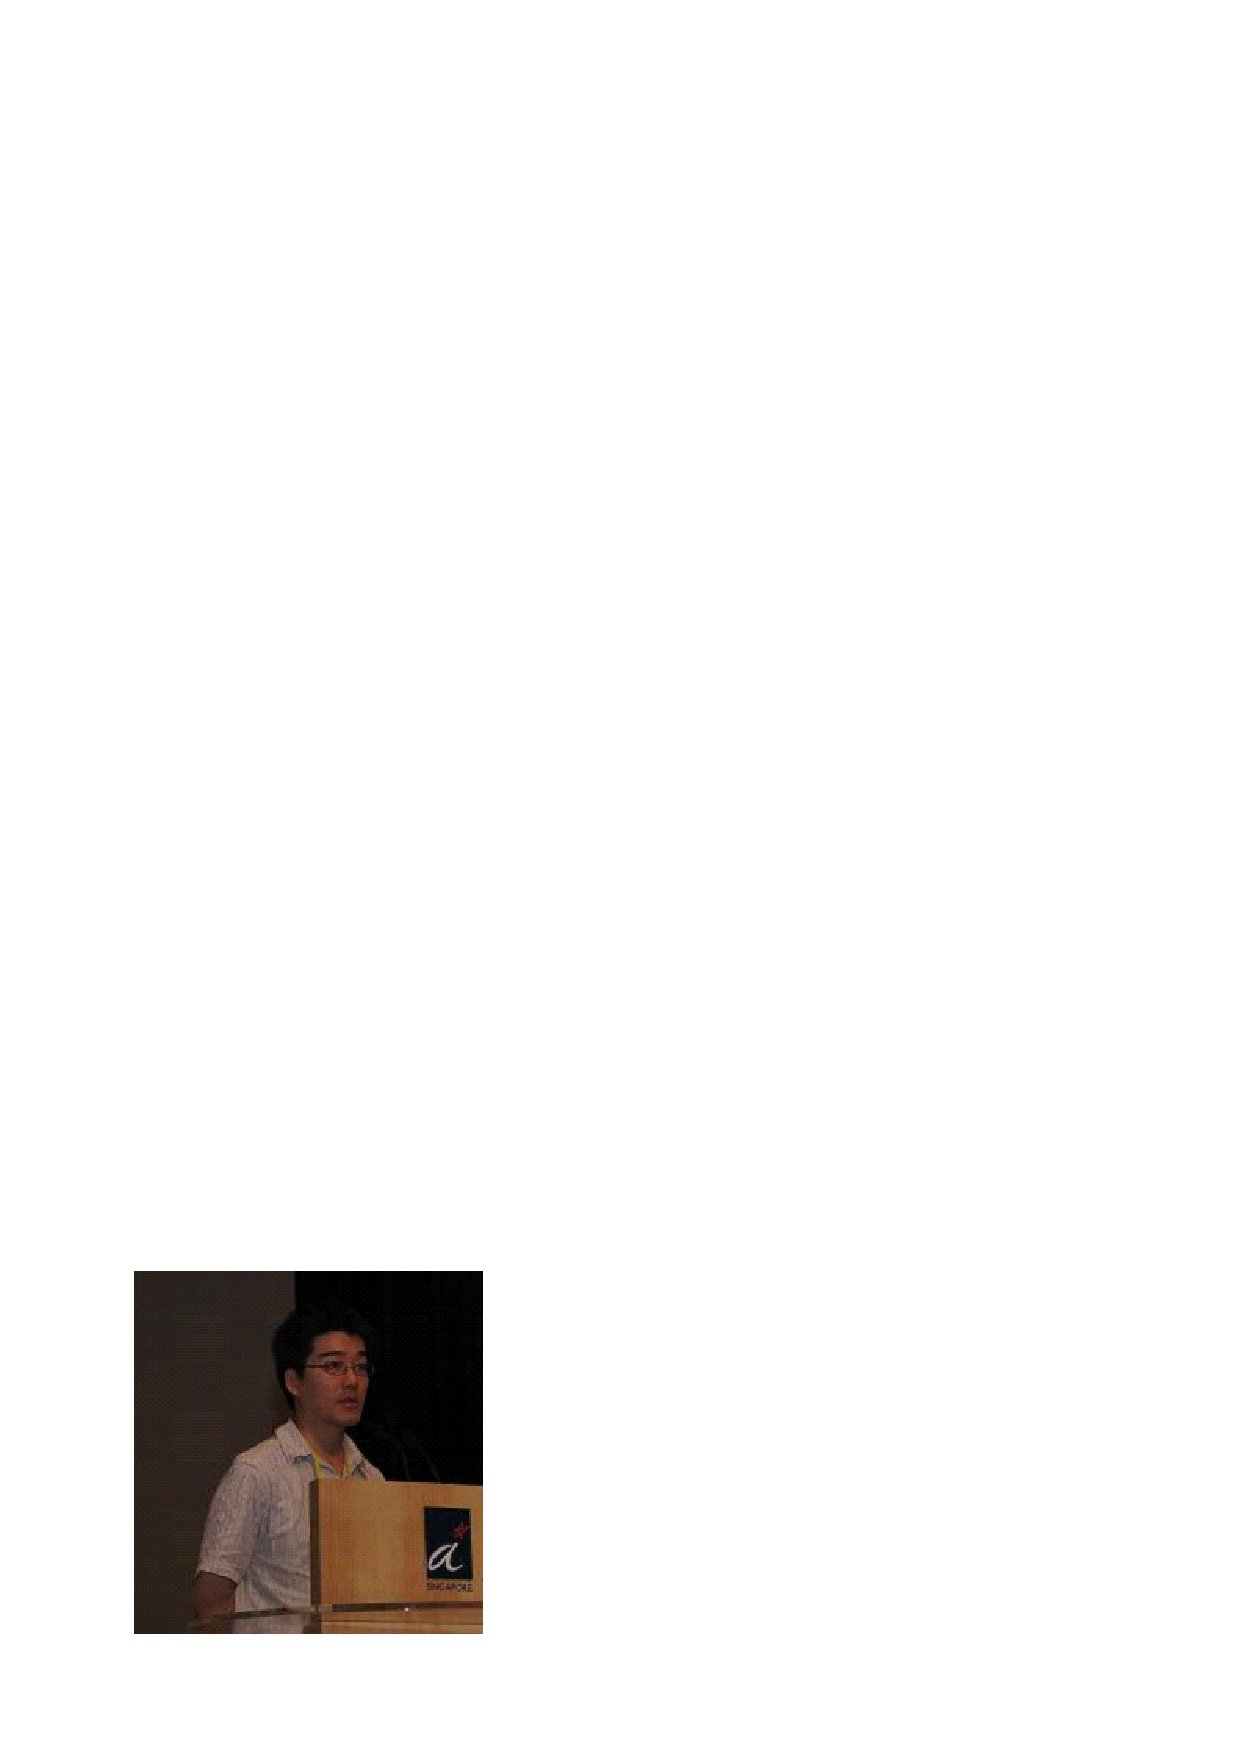
\includegraphics[scale=0.7]{profile1_2}
\end{center}
\vspace{9em}
\end{minipage}

\newpage

\section{Researches}

\subsection{Characterization of non-coding genomic regions}

\begin{figure}
\begin{center}
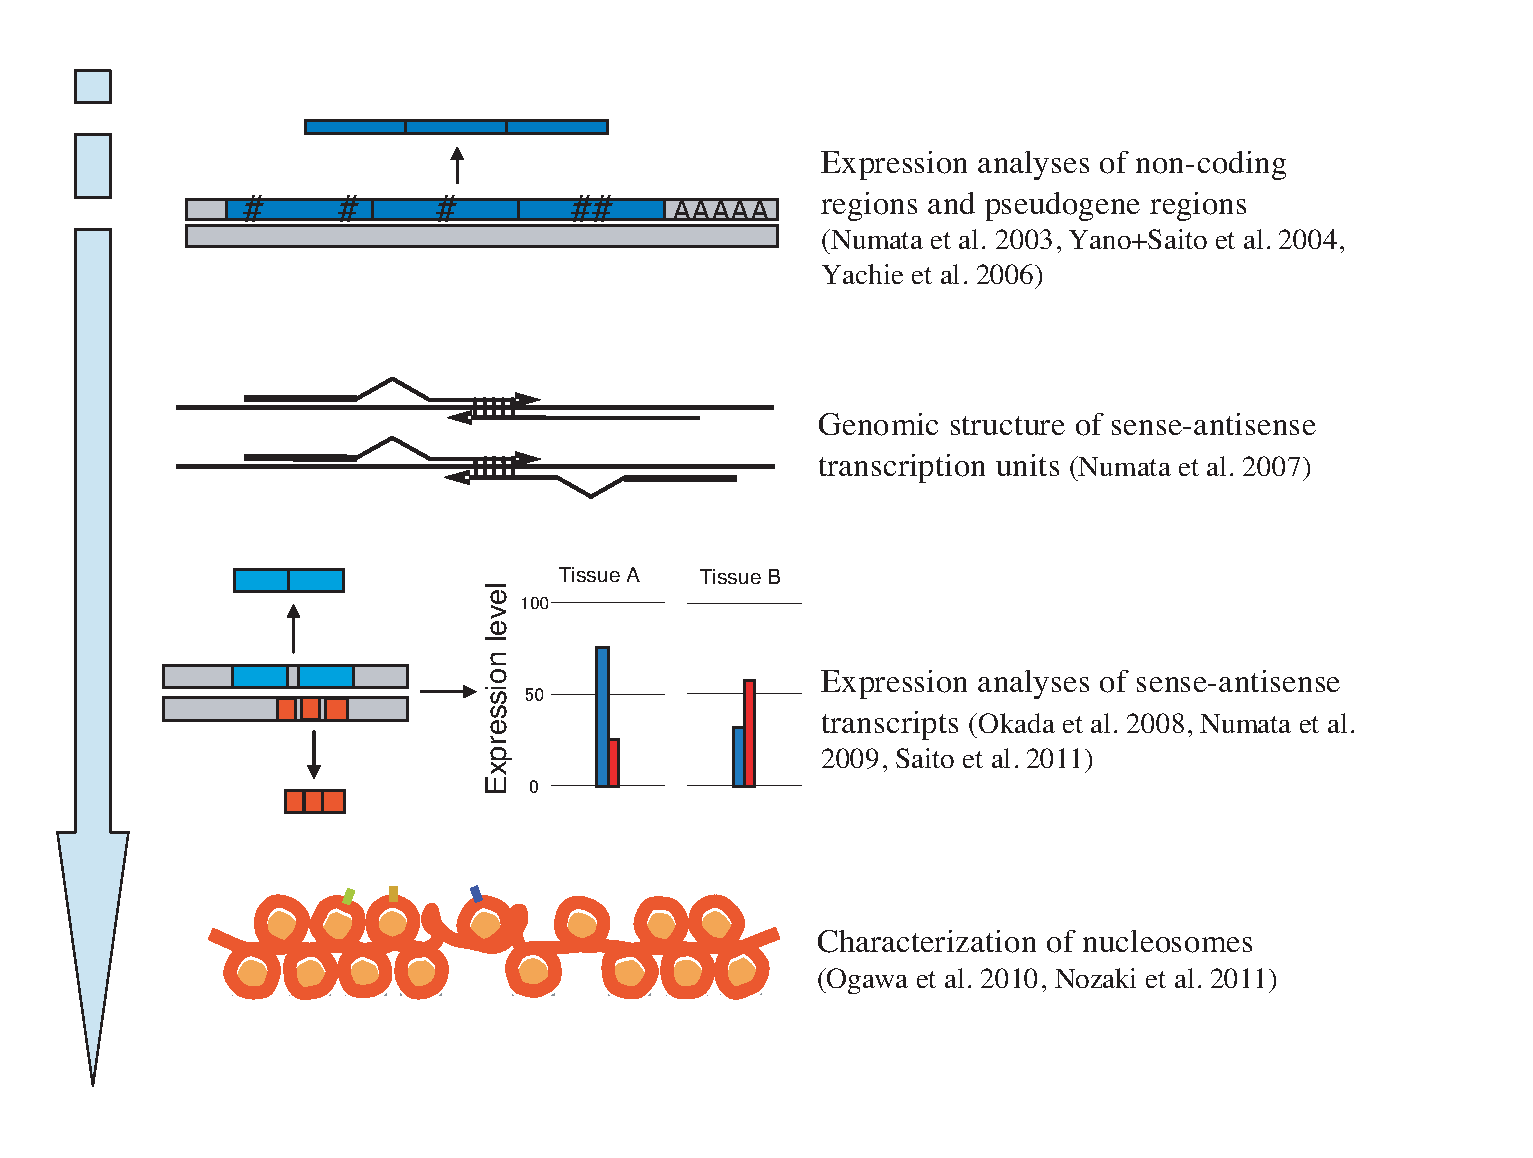
\includegraphics[scale=0.6]{research_ovv_RNA2}
\end{center}
\vspace{-1em}
\caption{History of our research on genome sequence analyses}
\label{research_ovv_RNA}
\end{figure}

Genomic sequences contain not only genes but also their regulatory 
information as well as information about how the organisms have evolved 
at the molecular level. We have especially been focusing on non-coding 
regions of the genomes and worked on 
computational characterization of these regions to investigate their 
functionality and to find how they have emerged (Figure \ref{research_ovv_RNA}) .

Although the human genome contains \(>97\%\) of non-protein-coding regions, 
their functions remain unclear. Our first step was to demonstrate that much of
these regions are transcribed. After joining the FANTOM project at RIKEN 
Genomic Sciences Center, we computationally analyzed 60,770 of mouse 
full-length cDNA sequences and surprisingly found that there are 
thousands of non-coding transcripts which do not encode proteins in the cell [\ref{pnc24},\ref{pnc34}]. Our analyses 
also showed that at least a small percentage of pseudogenes, which had been 
thought as inactive gene fossils, are expressed in human and mouse cell 
[\ref{pnc21}]. Subsequently, we developed a computational method (based 
on markov model which can assess RNA folding potential) to predict 
non-coding RNAs in {\it E. coli} [\ref{pnc17}].  The expression of some of 
non-coding RNA candidates predicted by our method was experimentally 
validated by RT-PCR and Northern blotting. 

Our next focus was characterization of antisense RNAs in various species, 
as we have found that some of non-coding predicted RNAs were encoded 
in the antisense strand of protein-coding genes [\ref{pnc17}]. We mapped 
cDNA sequences onto the genomes to find that there are thousands of such 
sense-antisense structures in various species [\ref{pnc13}]. We then 
analyzed expression patterns of these sense-antisense transcripts using 
our custom microarray [\ref{pnca1},\ref{pnca3},\ref{pnc4},\ref{pnc8}]. We designed 
microarray probes specific to the antisense strand of known genes and 
discovered hundreds of novel antisense transcripts in human and mouse. 
The expression levels of some of them were significantly altered in several 
tissues including cancer tissues, giving insights into the roles of 
these antisense transcripts.

We are now integrating epigenetic information to 
characterize genomic sequences; nowadays, a huge amount of epigenetic 
information about DNA methylations and histone modifications is 
available. 
We started with computational prediction 
of nucleosome positions on the genomes based on genomic sequence 
patterns [\ref{pnc2}].
We are analyzing correlations between genomic 
modification patterns, genomic features and features of transcripts encoded in the 
corresponding genomic region [\ref{pnca2}]. 

In addition, we are also interested in translation signals in 
mRNA sequences which was my main research focus during my doctoral 
course in the late 1990's. We found characteristic sequence patterns 
around start codons which are related to the mechanism and evolution of 
translation initiation [\ref{pnc46}].  We have extended these analyses to 
characterization of translation initiation signals using free energy 
[\ref{pnc45}] and information theory [\ref{pnc15}].  We also have worked 
on computational analyses of translation termination signals 
[\ref{pnc28},\ref{pnc32}], codon biases [\ref{pnc5}, \ref{pnc9}, 
\ref{pnc19}, \ref{pnc20}] and upstream Open Reading Frames (ORFs) [\ref{pnc10}].

\vspace{2em}

\noindent
{\large \bf Related publications}\\

\begin{small}
$^{\textcolor{red}{*}}$ Marked authors contributed equally to the work, $^{\textcolor{red}{+}}$ Corresponding author.
All reviewed by referees.
\end{small}

\begin{enumerate}

\item \label{pnca1} 
\underline{Saito R}$^{\textcolor{red}{*}}$, Kohno K$^{*}$, Okada Y, Osada Y, Numata K, Kohama C, Watanabe K, 
Nakaoka H, Yamamoto N, Kanai A, Yasue H, Murata S, Abe K, Tomita M, 
Ohkohchi N, Kiyosawa H (2011) 
{\bf Comprehensive Expressional Analyses of Antisense Transcripts in Colon Cancer Tissues Using Artificial Antisense Probes}. 
{\it BMC Medical Genomics} (accepted) 

\item \label{pnca2} 
Nozaki T, Yachie N, Ogawa R, \underline{Saito R}$^{\textcolor{red}{+}}$, Tomita M (2011) 
{\bf Computational analysis suggests a highly bendable, fragile structure for nucleosomal DNA}. {\it Gene} (in press) 

\item \label{pnca3} 
Watanabe Y, Numata K, Murata S, Osada Y, \underline{Saito R}, 
Nakaoka H, Yamamoto N, Watanabe K, Kato H, Abe K, Kiyosawa H (2010) 
{\bf Genome-wide analysis of expression modes and DNA methylation status at sense-antisense transcript loci in mouse}. 
{\it Genomics} 96(6):333-41 

\item \label{pnc1} Kratz A, Arner E, \underline{Saito R}, Kubosaki A, Kawai J, Suzuki H,
Carninci P, Arakawa T, Tomita M, Hayashizaki Y, Daub CO.
{\bf Core promoter structure and genomic context reflect histone 3
lysine 9 acetylation patterns}. {\it BMC Genomics} 11:257

\item \label{pnc2} Ogawa R, Kitagawa N, Ashida H, \underline{Saito R}$^{\textcolor{red}{+}}$, Tomita M(2010)
{\bf Computational prediction of nucleosome positioning by calculating the
relative fragment frequency index of nucleosomal sequences}.
{\it FEBS Let} 584(8):1498-502

\item \label{pnc4} Numata K, Osada Y, Okada Y, \underline{Saito R}, Hiraiwa N, 
Nakaoka H, Yamamoto N, Watanabe K, Okubo K, Kohama C, Kanai A, Abe K, 
Kiyosawa H.(2009) {\bf Identification of novel endogenous antisense 
transcripts by DNA microarray analysis targeting complementary strand of 
annotated genes}. {\it BMC Genomics} 10:392

\item \label{pnc5} Suzuki H, \underline{Saito R}$^{\textcolor{red}{+}}$, Tomita M.(2009) {\bf Measure of 
synonymous codon usage diversity among genes in bacteria}. {\it BMC 
Bioinformatics} 10:167.

\item \label{pnc6} FANTOM Consortium, Suzuki H, 
\(\cdots\)103 authors\(\cdots\),
\underline{Saito R}, 
\(\cdots\)32 authors\(\cdots\),
Hume DA;
Riken Omics Science Center, Arakawa T, 
\(\cdots\)20 authors\(\cdots\),
Hayashizaki 
Y.(2009) {\bf The transcriptional network that controls growth arrest and 
differentiation in a human myeloid leukemia cell line}. {\it Nat Genet}
41(5):553-62.

\item \label{pnc8} Okada Y, Tashiro C, Numata K, Watanabe K, Nakaoka H, Yamamoto N, 
Okubo K, Ikeda R, \underline{Saito R}$^{\textcolor{red}{+}}$, Kanai A, 
Abe K, Tomita M, Kiyosawa H$^{+}$ (2008) {\bf Comparative expression analysis 
uncovers novel features of endogenous antisense transcription}. {\it Hum Mol 
Genet} 17(11):1631-40

\item \label{pnc9} Suzuki H, \underline{Saito R}$^{\textcolor{red}{+}}$, Tomita M 
(2007) {\bf Variation in the Correlation of G + C Composition with Synonymous 
Codon Usage Bias among Bacteria}. {\it EURASIP J Bioinform Syst Biol} 61374

\item \label{pnc10} Matsui M, Yachie N, Okada Y, \underline{Saito 
R}$^{\textcolor{red}{+}}$, Tomita M.(2007) {\bf Bioinformatic analysis of 
post-transcriptional regulation by uORF in human and mouse}. {\it FEBS Let} 
581(22):4184-8

\item \label{pnc12} Arakawa K, \underline{Saito R}$^{\textcolor{red}{+}}$, Tomita M. 
(2007) {\bf Noise-reduction filtering for accurate detection of replication 
termini in bacterial genomes}. {\it FEBS Let} 581(2):253-8

\item \label{pnc13} Numata K, Okada Y, \underline{Saito R}$^{\textcolor{red}{+}}$, 
Kiyosawa H, Kanai A, Tomita M. (2007) {\bf Comparative analysis of 
cis-encoded antisense RNAs in eukaryotes}. {\it Gene} 392(1-2):134-41

\item \label{pnc14} Mori K, \underline{Saito R}$^{\textcolor{red}{+}}$, Kikuchi S$^{+}$, 
Tomita M (2006) {\bf Inferring rules of {\it E. coli} translational efficiency 
using an artificial neural network}. {\it Biosystems} 90(2):414-420 

\item \label{pnc15} Osada Y, \underline{Saito R}$^{\textcolor{red}{+}}$, Tomita M 
(2006) {\bf Comparative analysis of base correlations in 5' untranslated 
regions of various species}. {\it Gene} 375:80-6


\item \label{pnc17} Yachie N, Numata K, \underline{Saito R}$^{\textcolor{red}{+}}$, 
Kanai A, Tomita M (2006) {\bf Prediction of non-coding and antisense RNA 
genes in {\it Escherichia coli} with Gapped Markov Model}. {\it Gene} 372:171-81

\item \label{pnc18} Watanabe Y, Yachie N, Numata K, \underline{Saito R}, Kanai A, and 
Tomita M (2005) {\bf Computational analysis of microRNA target recognition in 
{\it Caenorhabditis elegans}}. {\it Gene} 365:2-10


\item \label{pnc19} Suzuki H, \underline{Saito R}$^{\textcolor{red}{+}}$, Tomita 
M.(2005) {\bf A problem in multivariate analysis of codon usage data and a 
possible solution}. {\it FEBS let} 579(28):6499-504


\item \label{pnc20} Suzuki H, \underline{Saito R}$^{\textcolor{red}{+}}$, Tomita 
M.(2004) {\bf The 'weighted sum of relative entropy': a new index for 
synonymous codon usage bias}. {\it Gene}. 335:19-23.


\item \label{pnc21} Yano Y*, \underline{Saito R}$^{\textcolor{red}{*}}$, Yoshida N, 
Yoshiki A, Wynshaw-Boris A, Tomita M, Hirotsune S(2004) {\bf A new role for 
expressed pseudogenes as ncRNA: regulation of mRNA stability of its 
homologous coding gene}. {\it J Mol Med} 82(7):414-22


\item \label{pnc22} Kikuchi S, 
\(\cdots\)64 authors\(\cdots\),
\underline{Saito R},
Sasaki D, Sato K, Shibata K, Shinagawa A, Shiraki T, Yoshino M,
Hayashizaki Y; Rice 
Full-Length cDNA Consortium; National Institute of Agrobiological 
Sciences Rice Full-Length cDNA Project Team; Foundation of Advancement 
of International Science Genome Sequencing \verb+&+ Analysis Group; 
RIKEN. (2003) {\bf Collection, mapping, and annotation of over 28,000 cDNA 
clones from japonica rice}. {\it Science} 301(5631):376-9.

\item \label{pnc23} Carninci P, Waki K, Shiraki T, Konno H, Shibata K, Itoh M, Aizawa 
K, Arakawa T, Ishii Y, Sasaki D, Bono H, Kondo S, Sugahara Y, 
\underline{Saito R}, 
\(\cdots\)32 authors\(\cdots\),
Hayashizaki Y. (2003) 
{\bf Targeting a complex transcriptome: the construction of the mouse 
full-length cDNA encyclopedia}. {\it Genome Res} 13(6B):1273-89

\item \label{pnc24} Numata, K., Kanai, A., \underline{Saito R}., Kondo, S., Adachi, J., 
Wilming L. G., Hume, D. A., RIKEN GER Group Members, Hayashizaki, Y. and 
Tomita, M.(2003) {\bf Identification of putative non-coding RNAs amongst the 
RIKEN mouse full-length cDNA collection}. {\it Genome Res} 13(6B):1301-1306.


\item \label{pnc25} Furuno M, Kasukawa T, \underline{Saito R}, Adachi J, Suzuki H, 
Baldarelli R, Hayashizaki Y, Okazaki Y.(2003) {\bf CDS annotation in 
full-length cDNA sequence}. {\it Genome Res} 13(6B):1478-87.


\item \label{pnc26} Nagashima T, Silva DG, Petrovsky N, Socha LA, Suzuki H, 
\underline{Saito R}, Kasukawa T, Kurochkin IV, Konagaya A, Schonbach 
C.(2003) {\bf Inferring higher functional information for RIKEN mouse 
full-length cDNA clones with FACTS}. {\it Genome Res} 13(6B):1520-33.

\item \label{pnc28} Ozawa, Y., \underline{Saito R}., Washio, T, and Tomita, M.(2003) 
{\bf Comparative study of translation termination sites and release factors 
(RF1 and RF2) in prokaryotes}. {\it J Mol Evol} 56(6):665-72

\item \label{pnc29} Sato, M., Umeki, H., \underline{Saito R}$^{\textcolor{red}{+}}$, 
Kanai, A. and Tomita, M. (2003) {\bf Computational analysis of stop codon 
readthrough in {\it D. melanogaster}}. {\it Bioinformatics} 19(11):1371-80

\item \label{pnc32} Ozawa Y, Hanaoka S, \underline{Saito R}, Washio T, Nakano S, 
Shinagawa A, Itoh M, Shibata K, Carninci P, Konno H, Kawai J, 
Hayashizaki Y, Tomita M.(2002) {\bf Comprehensive sequence analysis of 
translation termination sites in various eukaryotes}. {\it Gene} 300(1-2):79-87.

\item \label{pnc33} Sakurai A, Fujimori S, Kochiwa H, Kitamura-Abe S, Washio T, 
\underline{Saito R}, Carninci P, Hayashizaki Y, Tomita M. (2002) {\bf On 
biased distribution of introns in various eukaryotes}. {\it Gene} 
300(1-2):89-95.


\item \label{pnc34} Okazaki Y, Furuno M, Kasukawa T, Adachi J, Bono H, Kondo 
S, Nikaido I, Osato N, \underline{Saito R},
%Suzuki H, Yamanaka I, Kiyosawa H, 
%Yagi K, Tomaru Y, Hasegawa Y, Nogami A, 
%Schonbach C, Gojobori T, Baldarelli R, Hill DP, Bult C, Hume, 
%DA, Quackenbush J, Schriml LM, Kanapin A, Matsuda H, 
%Batalov S, Beisel KW, Blake JA, Bradt D, Brusic V,
%Chothia C, Corbani LE, Cousins S, Dalla E, Dragani TA, Fletcher CF,
%Forrest A, Frazer KS, Gaasterland T, Gariboldi M, Gissi C, 
%Godzik A, Gough J, Grimmond S, Gustincich S, Hirokawa N, 
%Jackson IJ, Jarvis ED, Kanai A, Kawaji H, Kawasawa Y, 
%Kedzierski RM, King BL, Konagaya A, Kurochkin IV, Lee Y, 
%Lenhard B, Lyons PA, Maglott DR, Maltais L, Marchionni L, 
%McKenzie L, Miki H, Nagashima T, Numata K, Okido T, Pavan WJ,
%Pertea G, Pesole G, Petrovsky N, Pillai R, Pontius JU, 
%Qi D, Ramachandran S, Ravasi T, Reed JC, Reed DJ, Reid J, 
%Ring BZ, Ringwald M, Sandelin A, Schneider C, Semple CA, 
%Setou M, Shimada K, Sultana R, Takenaka Y, Taylor MS, 
%Teasdale RD, Tomita M, Verardo R, Wagner L, Wahlestedt C, 
%Wang Y, Watanabe Y, Wells C, Wilming LG, Wynshaw-Boris A, 
%Yanagisawa M, Yang I, Yang L, Yuan Z, Zavolan M, Zhu Y, 
%Zimmer A, Carninci P, Hayatsu N, Hirozane-Kishikawa T, Konno H, 
%Nakamura M, Sakazume N, Sato K, Shiraki T, Waki K, Kawai J, 
%Aizawa K, Arakawa T, Fukuda S, Hara A, Hashizume W, Imotani K, 
%Ishii Y, Itoh M, Kagawa I, Miyazaki A, Sakai K, Sasaki D, 
%Shibata K, Shinagawa A, Yasunishi A, Yoshino M, Waterston R, 
%Lander ES, Rogers J, Birney E,
\(\cdots\)128 authors\(\cdots\),
Hayashizaki Y 
(2002) {\bf Analysis of the mouse transcriptome based on functional 
annotation of 60,770 full-length cDNAs}. {\it Nature 420}: 563-573. 


\item \label{pnc35} Kochiwa H, Suzuki R, Washio T, \underline{Saito R}, Bono H, 
Carninci P, Okazaki Y, Miki R, Hayashizaki Y, Tomita, M.
(2002) {\bf Inferring alternative splicing patterns in mouse from a 
full-length cDNA library and microarray data}. {\bf Genome Res} 12(8): 1286-93

\item \label{pnc39} Sakai H, Washio T, \underline{Saito R}, Shinagawa A, Itoh M,
Shibata K, Carninci P, Konno H, Kawai J, Hayashizaki Y, Tomita M.(2001)
 {\bf Correlation between sequence conservation of the 5' 
untranslated region and codon usage bias in {\it Mus musculus} genes}. {\it Gene} 
276(1-2): 101-5.


\item \label{pnc40} Sakai H, Imamura C, Osada Y, \underline{Saito R}, Washio T, 
Tomita M.(2001) {\bf Correlation between Shine-Dalgarno sequence 
conservation and codon usage of bacterial genes}. {\it J Mol Evol} 52(2): 
164-70.


\item \label{pnc41} Kawai J,
%Shinagawa A, Shibata K, Yoshino M,
%Itoh M, Ishii Y, Arakawa T, Hara A, Fukunishi Y, Konno H,
%Adachi J, Fukuda S, Aizawa K, Izawa M, Nishi K, Kiyosawa H, Kondo S, 
%Yamanaka I, Saito T, Okazaki Y, Gojobori T, Bono H, Kasukawa T, 
\(\cdots\)22 authors\(\cdots\),
\underline{Saito R},
%Kadota K, Matsuda H, Ashburner M, Batalov S, 
%Casavant T, Fleischmann W, Gaasterland T, Gissi C, King B, 
%Kochiwa H, Kuehl P, Lewis S, Matsuo Y,  Nikaido I, Pesole G, 
%Quackenbush J, Schriml LM, Staubli F, Suzuki R, Tomita M, 
%Wagner L, Washio T, Sakai K, Okido T, Furuno M, Aono H, 
%Baldarelli R, Barsh G, Blake J, Boffelli D, Bojunga N,
%Carninci P, de Bonaldo MF, Brownstein MJ, Bult C,
%Fletcher C, Fujita M, Gariboldi M, Gustincich S, Hill D,
%Hofmann M, Hume DA, Kamiya M, Lee NH, Lyons P, Marchionni L, Mashima J, 
%Mazzarelli J, Mombaerts P, Nordone P, Ring B,  Ringwald M, 
%Rodriguez I, Sakamoto N, Sasaki H, Sato K, Schonbach C,
%Seya T, Shibata Y, Storch KF, Suzuki H, Toyo-oka K, Wang KH, 
%Weitz C, Whittaker C, Wilming L, Wynshaw-Boris A, Yoshida K, 
%Hasegawa Y, Kawaji H, Kohtsuki S,
\(\cdots\)71 authors\(\cdots\),
Hayashizaki Y (2001) 
{\bf Functional annotation of a full-length mouse cDNA collection}. {\it Nature}
409: 685-90.


\item \label{pnc42} \underline{Saito R}, Ozawa Y, Kuzuno N, Tomita M (2000) 
{\bf Computer analysis of potential stem structures of�@rRNA operons in 
various procaryote genomes}. {\it Gene} 259(1-2): 217-22.


\item \label{pnc43} Toda Y, \underline{Saito R}, Tomita M (2000) 
{\bf Characteristic sequence pattern in the 5- to 20-bp upstream region of 
primate {\it Alu} elements}. {\it J Mol Evol} 50(3):232-7.


\item \label{pnc44} \underline{Saito R}, Tomita M (1999) {\bf Computer analyses of 
complete genomes suggest that some archaebacteria employ both eukaryotic 
and eubacterial mechanisms in translation initiation}. {\it Gene} 238(1): 
79-83.


\item \label{pnc45} Osada Y, \underline{Saito R}, Tomita M (1999) {\bf Analysis of 
base-pairing potentials between 16S rRNA and 5' UTR for translation 
initiation in various prokaryotes}. {\it Bioinformatics} 15(7-8): 578-81.

\item \label{pnc46} \underline{Saito R}, Tomita M (1999) {\bf On negative selection 
against ATG triplets near start codons in eukaryotic and prokaryotic 
genomes}. {\it J Mol Evol} 48(2): 213-7.

\label{pnc_last}
\end{enumerate}



\subsection{Interactome analyses}

\begin{figure}
\begin{center}
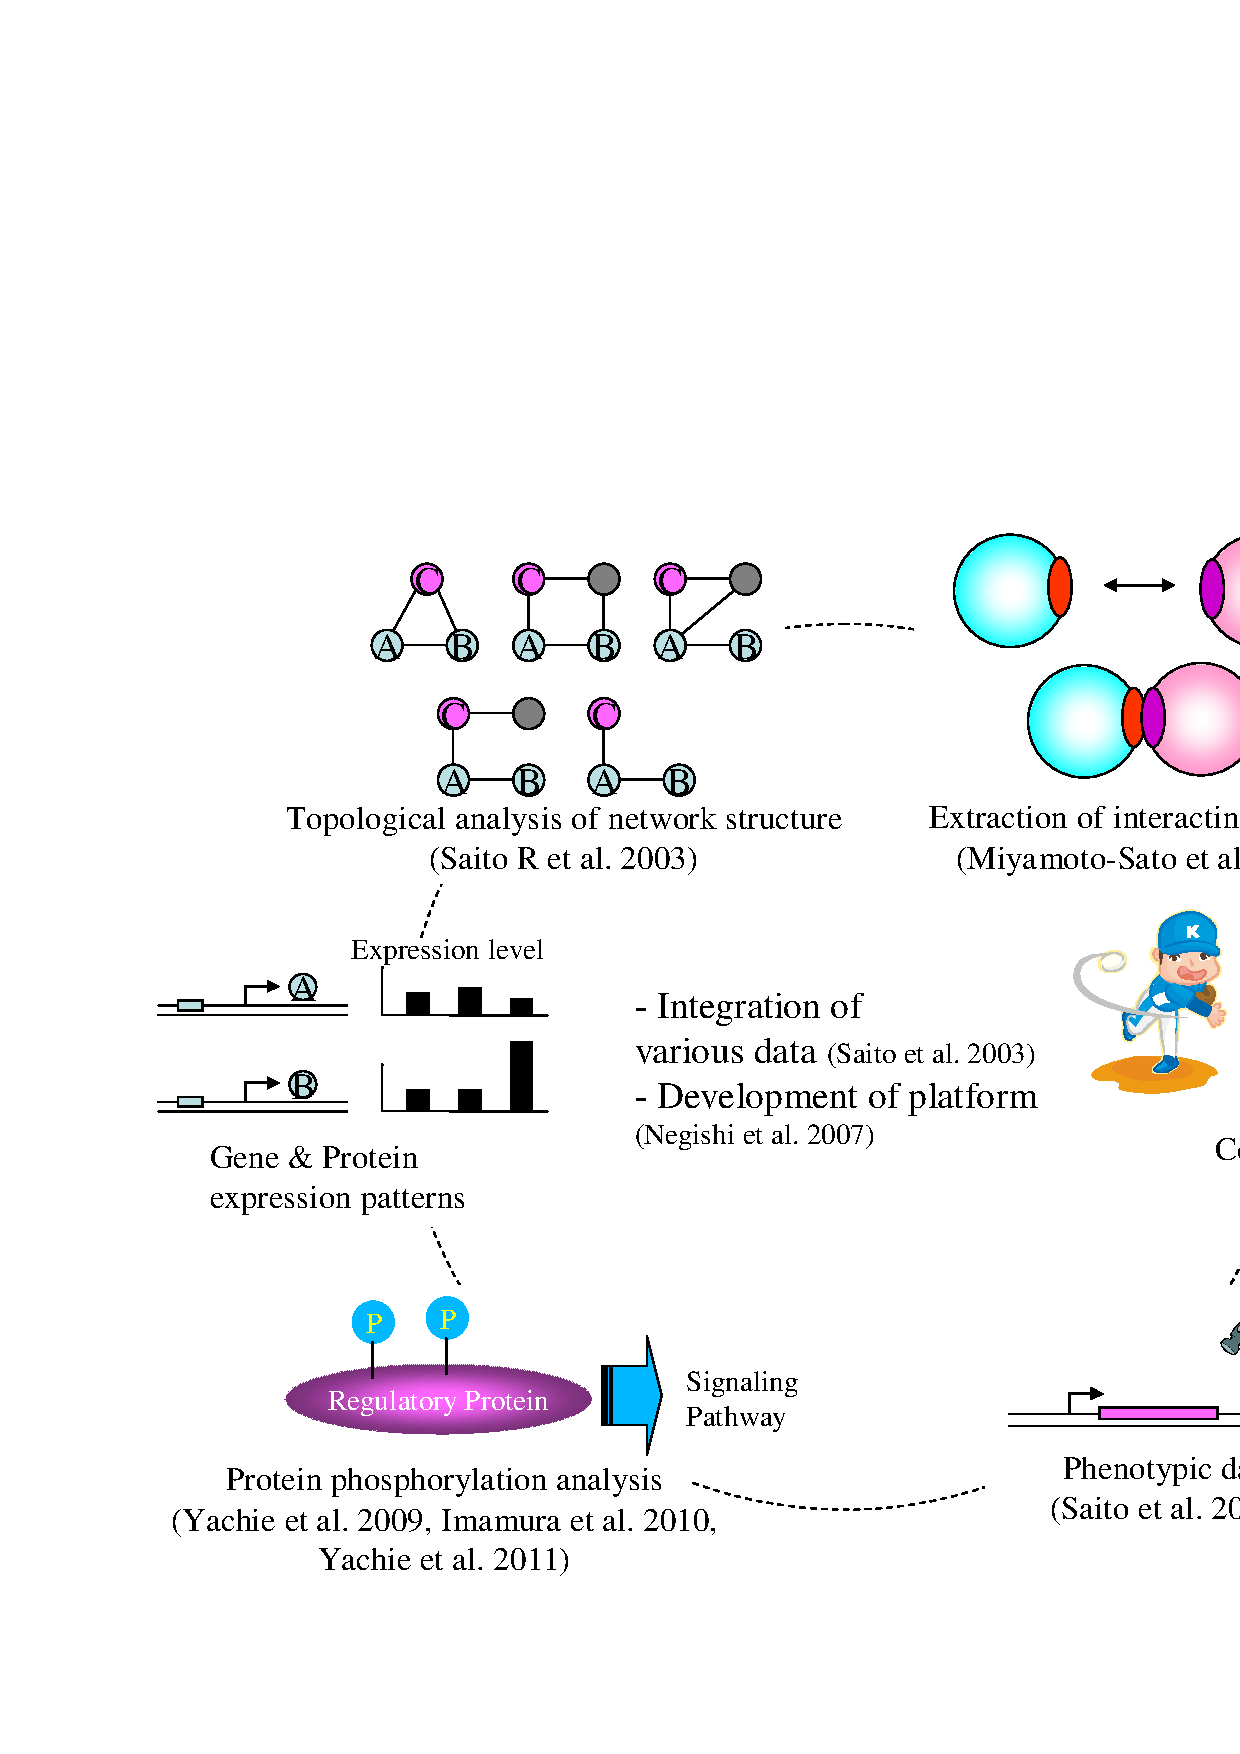
\includegraphics[scale=0.6]{research_ovv_PPI2}
\end{center}
\vspace{-1em}
\caption{Interactome analysis through integration of various data and techniques}
\label{research_ovv_PPI}
\end{figure}

Recent high-throughput technologies such as the yeast two-hybrid system 
allowed to obtain information about a very large number of molecular 
interactions (mainly protein-protein interactions) in a cell. We have 
been working on computational analyses of such large interaction datasets to 
extract valuable functional information from them. The research started in 2000 
with development of methods to eliminate false positives from 
protein-protein interaction (PPI) data - one of the main problems in 
dealing with high-throughput PPI data was the large amount of false positives 
within these datasets. Using topological features which are frequently 
observed in spurious interactions, we developed methods to eliminate 
these false positives [\ref{itr30},\ref{itr36}].

% This allowed us to predict functions of
% uncharacterized proteins more efficiently.

The next step was to integrate PPI data with other types of genome-wide 
data. We first integrated PPI data with genome-wide expression data to 
find that similarity in expression pattern supports true PPI. Then we 
integrated phenotypic data (lethality of gene deletion) to find that 
proteins participating in specific interactions are likely to have 
similar phenotypes [\ref{itr31}].

As various genome-wide data became available, we further attempted
to efficiently integrate these data to extract novel biological knowledge
(Figure \ref{research_ovv_PPI}), keeping computational prediction of novel signal
transduction pathways as our final goal. To do so, we first looked for 
genome-wide data which we should integrate. 

Domain-domain interaction data were one of the candidates. We 
collaborated with experimental group using {\it in vitro} virus (IVV) 
technology to identify novel protein binding domains [\ref{itr3}]. By 
combining the IVV data with our computational methods, we predicted not 
only PPIs but also their domain-domain interactions, some of which were 
validated by pull-down assay ([\ref{itr_cmplx1}], Manuscript in preparation).

As PPI networks are usually represented as un-directed graph, it is 
difficult to infer signaling pathway from these data because signaling 
pathways are usually "directed". Recent development in mass spectrometry 
allowed to obtain genome-wide protein phosphorylation status data which can be used to 
assign signaling directions from kinase to substrates within
signaling pathways. We began to computationally characterize 
phosphorylation sites in phospho-protein sequences and found the 
"rich-gets-richer" process (phospho-proteins having many phospho-sites 
are likely to gain more phospho-sites) during molecular evolution of 
phospho-proteins [\ref{itr7}]. We also developed preliminary methods to 
roughly draw signaling pathways based on time-course data of 
phosphorylation patterns [\ref{itr_hi1}].

To integrate, analyze and visualize various kind of genome-wide data, 
we have also developed a software platform, {\bf eXpanda}, which 
provides useful APIs for bioinformaticians to study interaction networks 
[\ref{itr11}].

\vspace{2em}

\noindent
{\large \bf Related publications}\\

\begin{small}
$^{\textcolor{red}{*}}$ Marked authors contributed equally to the work, $^{\textcolor{red}{+}}$ Corresponding author.
All reviewed by referees.
\end{small}

\begin{enumerate}
\setcounter{enumi}{\ref{pnc_last}} % Indicate the last previous publication.

\item \label{itra1}
Yachie N, \underline{Saito R}$^{\textcolor{red}{+}}$, Sugiyama N, Tomita M, Ishihama Y (2011) 
{\bf Integrative features of the yeast phosphoproteome and protein-protein interaction map}. {\it PLoS comput biol} 7(1):e1001064 

\item \label{itr_cmplx1} Ozawa Y, \underline{Saito R}$^{\textcolor{red}{+}}$, Fujimori S, Kashima H, 
Ishizaka M, Yanagawa H, Miyamoto-Sato E, Tomita M (2010) Protein complex 
prediction via verifying and reconstructing the topology of 
domain-domain interactions. BMC Bioinformatics (In press) 


\item \label{itr_hi1} Imamura H, Yachie N, \underline{Saito R}$^{\textcolor{red}{+}}$, Ishihama Y, Tomita M (2010)
{\bf Towards the systematic discovery of signal transduction networks using phosphorylation dynamics data}.
{\it BMC Bioinformatics} 11(1):232

\item \label{itr3} Miyamoto-Sato E, Fujimori S, Ishizaka M, Hirai N, Masuoka K, 
\underline{Saito R}, Ozawa Y, Hino K, Washio T, Tomita M, Yamashita T, 
Oshikubo T, Akasaka H, Sugiyama J, Matsumoto Y, Yanagawa H.(2010) {\bf A 
comprehensive  resource  of  interacting  protein  regions  for refining 
human transcription  factor  networks}. {\it PloS ONE} (In press)

\item \label{itr7} Yachie N, \underline{Saito R}$^{\textcolor{red}{+}}$, Sugahara J, 
Tomita M, Ishihama Y(2009) {\bf {\it In silico} analysis of phosphoproteome data 
suggests a rich-get-richer process of phosphosite accumulation over 
evolution}. {\it Mol Cell Proteomics} 8(5):1061-71.

\item \label{itr11} Negishi Y, Nakamura H, Yachie N, \underline{Saito 
R}$^{\textcolor{red}{+}}$, Tomita M (2007) {\bf eXpanda: an Integrated 
Platform for Network Analysis and Visualization}. {\it In silico biology} 7, 
0013

\item \label{itr16} Arifuzzaman M, Maeda M, Itoh A, Nishikata K, Takita C, 
\underline{Saito R}, Ara T, Nakahigashi K, Huang HC, Hirai A, Tsuzuki T, 
Nakamura S, Altaf-Ul-Amin M, Oshima T, Baba T, Yamamoto N, Kawamura T, 
oka-Nakamichi T, Kitagawa M, Tomita M, Kanaya S, Wada C, Mori H (2006) 
{\bf Large-scale identification of protein-protein interaction of {\it Escherichia 
coli} K-12} {\it Genome Res} 16(5):686-91

\item \label{itr27} Suzuki, H., \underline{Saito R}., Kanamori, M., Kai, C., Schonbach, 
C., Nagashima, T., Hosaka, J., Hayashizaki, Y.(2003) {\bf The mammalian 
protein-protein interaction database and its viewing system that is 
linked to the main FANTOM2 viewer}. {\it Genome Res} 13(6B):1534-1541.

\item \label{itr30} \underline{Saito R}., Suzuki, H., Hayashizaki, Y.(2003) 
{\bf Construction of reliable protein-protein interaction networks with a new 
interaction generality measure}. {\it Bioinformatics} 19(6):756-63.


\item \label{itr31} \underline{Saito R}, Suzuki H, Hayashizaki Y.(2003) {\bf Global 
insights into protein complexes through integrated analysis of the 
reliable interactome and knockout lethality}. {\it Biochem Biophys Res Commun} 
301(3):633-40.

\item \label{itr36} \underline{Saito R}., Suzuki, H. and Hayashizaki, Y. (2002) 
{\bf Interaction generality, a measurement to assess the reliability of a 
protein-protein interaction}. {\it Nucleic Acids Res} 30(5): 1163-8.

\item \label{itr37} Kanamori M, Suzuki H, \underline{Saito R}, Muramatsu M, 
Hayashizaki Y.(2002) {\bf T2BP, a Novel TRAF2 Binding Protein, Can Activate 
NF-kappaB and AP-1 without TNF Stimulation}. {\it Biochem Biophys Res Commun} 
290(3):1108-13.


\item \label{itr38} Suzuki H, Fukunishi Y, Kagawa I, \underline{Saito R}, Oda H, Endo 
T, Kondo S, Bono H, Okazaki Y, Hayashizaki Y.(2001) {\bf Protein-protein 
interaction panel using mouse full-length cDNAs}. {\it Genome Res}
11(10):1758-65.

\end{enumerate}


\section{Career}

\begin{tabular}{lcll}
1983.6 & - & 1986.5 & Hawthorne Elementary School (Ottawa Ontario, CANADA)\\
1986.6 & - & 1988.3 & Higashiyama Junior High School (Public school)\\
1988.4 & - & 1991.3 & Keio High School (Private school)\\
1991.4 & - & 1995.3 & Keio University Faculty of Environmental Information\\
       &   &        & (Bachelor's degree, 1995)\\
1995.4 & - & 1997.3 & Keio University Graduate School of Media and Governance Master Course\\
       &   &        & (Master's degree, 1997)\\
1997.4 & - & 2000.3 & Keio University Graduate School of Media and Governance Doctoral Course\\
       &   &        & (Ph.D., 2000)\\
       &   &        & Thesis title: "Computer Analyses of Translation Initiation Sites of Genes"\\
       &   &        & \\
2000.4 & - & 2002.3 & RIKEN Genomic Sciences Center (Researcher)\\
2002.4 & - & 2010.1 & Institute for Advanced Biosciences, Keio University (Assistant professor)\\
2010.2 & - &        & University of California, San Diego\\
       &   &        & Departments of Medicine and Bioengineering (Visiting Faculty)\\
\end{tabular}


\section{Experienced teaching classes}

\begin{description}
\item[Programing For Genome Analysis] \verb+ +\\
\vspace{-1.5em}
\begin{itemize}
\item Basic Perl/Python programming.
\item Basic analysis of genomic sequences.
\end{itemize}
\item[Genome Informatics] \verb+ +\\
\vspace{-1.5em}
\begin{itemize}
\item Basic mathematical statistics (Gaussian distribution, \(\chi^{2}\) distribution, etc.).
\item DNA/RNA sequence analysis using information theory (Derivation of entropy, mutual information, Kullback-Leibler divergence, etc. and their applications to DNA/RNA sequence analysis).
\item Prediction of RNA secondary structure by free energy optimization.
\end{itemize}
\item[Molecular And Cellular Biology 3] \verb+ +\\
\vspace{-1.5em}
\begin{itemize}
\item Chemical structure of membrane proteins.
\item Chemical network of energy metabolism.
\end{itemize}
\item[Bioinformatics Algorithms]\hspace{-0.5em}\footnote{This course is for graduate students} \verb+ +\\
\vspace{-1.5em}
\begin{itemize}
\item Basic theory on algorithms including recursion and \(O\)-notation.
\item Dynamic programming, sequence alignment.
\item Probabilistic models (Hidden Markov Model).
\item Machine-learning, maximum-likelihood method, Expectation-Maximization algorithm.
\item Hierarchical clustering, {\it k}-means clustering, self-organization map.
\end{itemize}
\end{description}


\section{Patent}

Assessment of Protein-Protein Interactions (JP-A-2003-194813 (P2003-194813A))
% �^���p�N���ԑ��ݍ�p�̕]�����@ (���J�Q�O�O�R�|�P�X�S�W�P�R�i�o�Q�O�O�R�|�P�X�S�W�P�R�`�j)



\section{Skills}

\begin{description}
\item[English] Fluent (Lived in Ottawa, Canada from 1983 to 1986.)
\item[Bioinformatics] Familiar with computational genomic sequence analysis
and protein-protein interaction analysis. Experienced analyzing many gene
expression data. Familiar with bioinformatics tools such as BLAST, FASTA, clustalw,
HMMer, RNAfold. Experienced using cytoscape.
\item[Programming] Python (Main), Perl (Familiar), C (Familiar), R, C++, 
Java, Prolog, Microsoft VBA, Bourne shell, Awk, etc.
% \item[Statistics] Familiar with statistical tests including \(Z\)-test, \(t\)-test, \(\chi^{2}\) test, etc. Experienced using principal component analysis, correspondence analysis,
% fourier transformation for my researches. Familiar with R language.
\item[Biological experiments] Experienced some basic techniques from 2003 to 2004 (RT-PCR, electrophoresis, Western Blotting, vector construction, transformation, etc.)
\end{description}


\newpage

\section{Book Publication}

\subsection{Fundamental Bioinformatics}

\begin{minipage}{0.45\hsize}
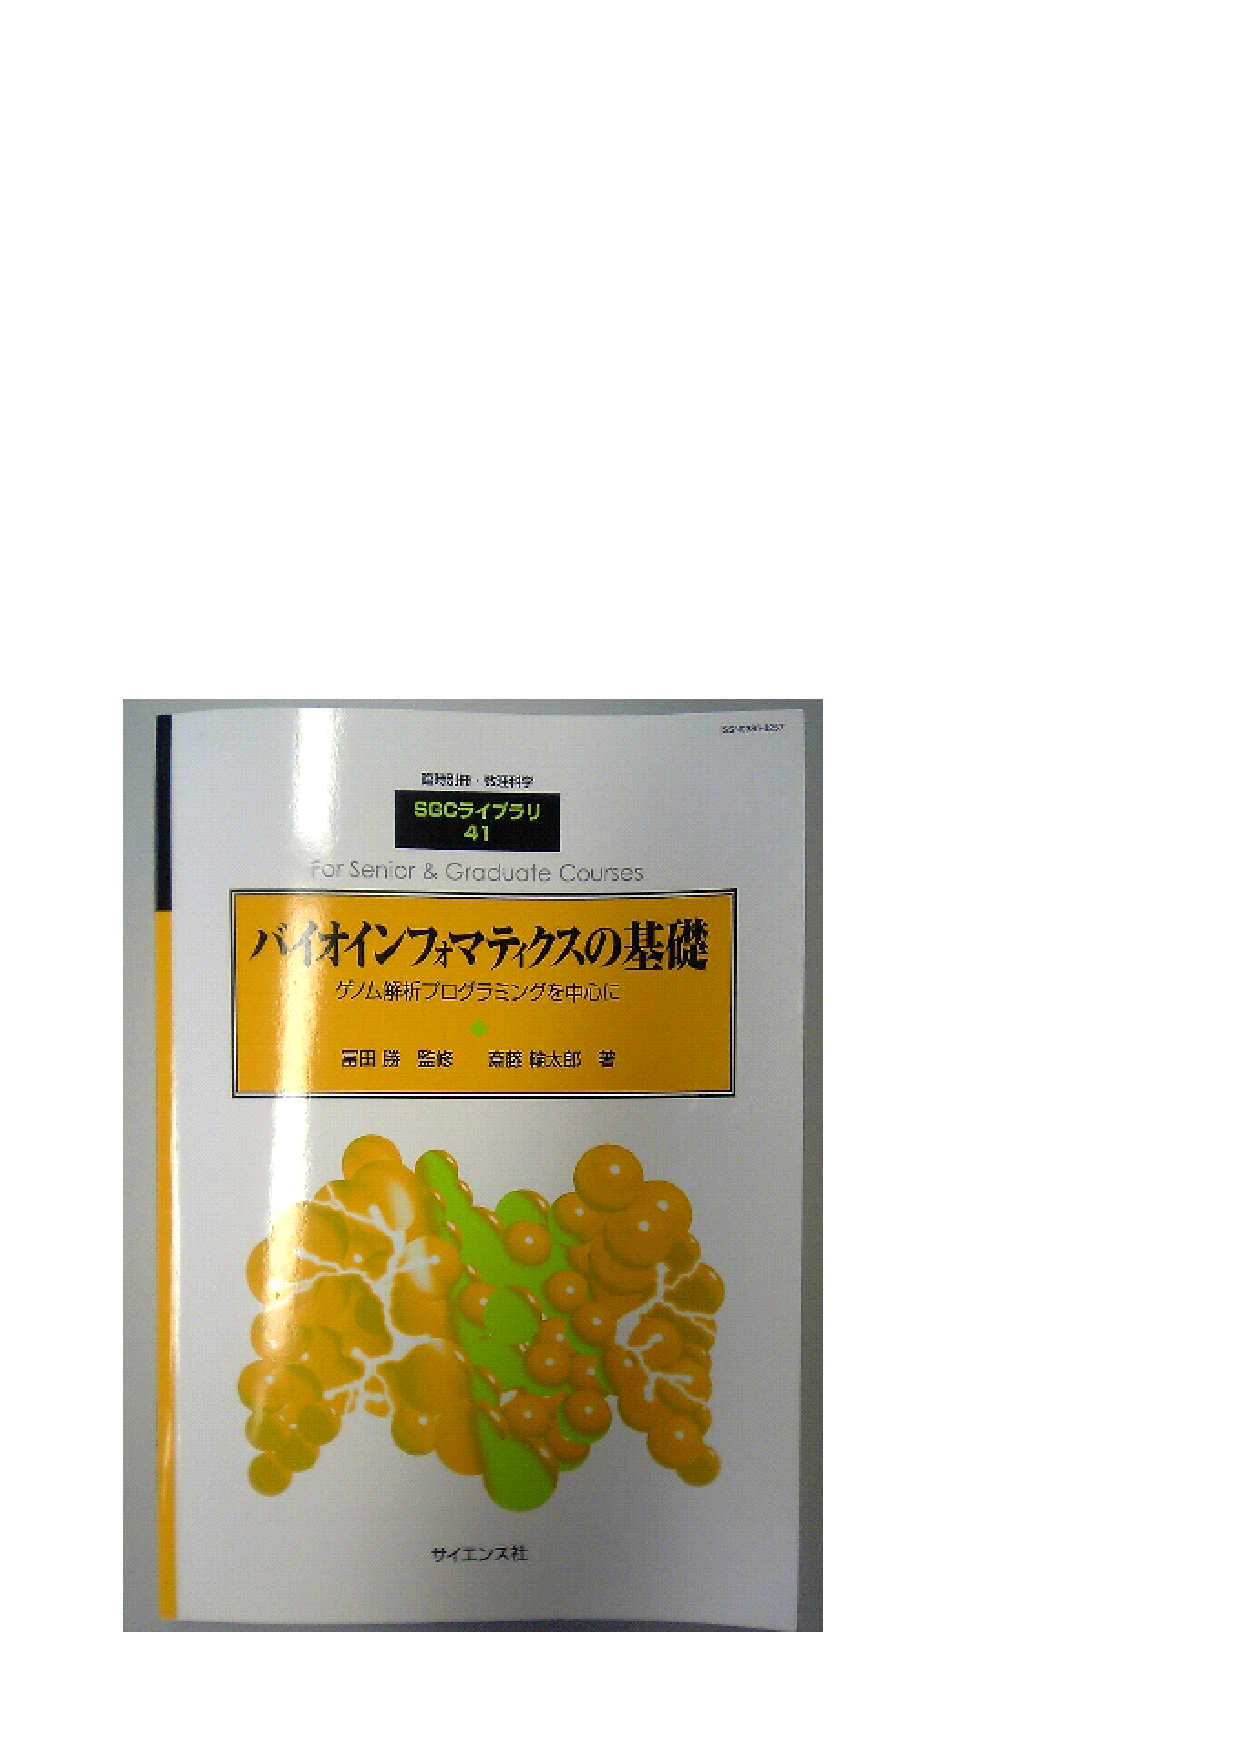
\includegraphics[scale=0.5]{bioinfo_book1}
\end{minipage}
\begin{minipage}{0.55\hsize}
\begin{description}
\item[Book title] Fundamental Bioinformatics\footnote{Translation for "Bioinformatics no kiso".}
\item[Book subtitle] Approach from genome analysis programming\footnote{Translation for "Genome kaiseki programming wo chushin ni".}
\item[Author] Rintaro Saito
\item[Supervisor] Masaru Tomita
\item[Published Date] 2005-07-25
\item[Publisher] Saiensu-sha Co., Ltd.
\item[Pages] 168
\item[Language] Japanese
\item[ISSN] 4910054700756
\end{description}
\end{minipage}

\vspace{1em}

{\bf Contents}
\begin{itemize}

\item Genome sequence analysis using information theory (Entropy,
  relative entropy, mutual information)
\item Statistics (\(Z\)-test, \(\chi^{2}\)-test)
\item Dynamic programming and application to sequence alignment
and prediction of RNA secondary structure (Derivation of Zuker's formula)
\item Hidden Markov Model, Viterbi's algorithm, forward and backward algorithms,
paramater estimation using Baum-Welch algorithm.
\item Hierarchical clustering and {\it k}-means clustering of gene expression data.
\item Analysis of codon biases using principal component analysis (PCA), correspondence analysis (CA) and
self-organization map (SOM). Mathematical derivation of PCA and CA.
\item Appendices
\begin{itemize}
\item Recursion, {\it O}-notation
\item Derivation of Gaussian distribution and \(\chi^{2}\) distribution.
\item Lagrange multipliers
\item Maximum likelihood estimation, expectation maximization algorithm
\end{itemize}
\end{itemize}

\newpage

\section{References}

\subsection*{Masaru Tomita, Ph.D.}
Director and Professor\\
Institute for Advanced Biosicences\\
Faculty of Environmental and Information Studies\\
Keio University\\
Tel: +81-466-47-5099\\
Fax: +81-466-47-5099\\
E-Mail: mt@sfc.keio.ac.jp\\
Web Page: http://www.iab.keio.ac.jp/en/content/view/34/124/

\subsection*{Yasushi Ishihama, Ph.D.} 
Associate Professor\\
Institute for Advanced Biosicences\\
Faculty of Environmental and Information Studies\\
Keio University\\
Tel: +81-235-29-0571\\
Fax: +81-235-29-0536\\
E-Mail: y-ishi@ttck.keio.ac.jp\\
Web Page: http://www.iab.keio.ac.jp/en/content/view/43/124/

\subsection*{Haruo Suzuki, Ph.D.}

Research Associate\\
Department of Population Medicine and Diagnostic Sciences\\
College of Veterinary Medicine\\
Cornell University\\
%Ithaca, NY 14853, USA
Tel: +1-607-253-4228\\
Fax: +1-607-256-5608\\
E-Mail: hs568@cornell.edu \\


\end{document}

